% !BIB program = biber

\documentclass[11pt, oneside]{report}

% set up some more document options
\usepackage[utf8]{inputenc}
\usepackage[parfill]{parskip}
\usepackage[english]{babel}
\usepackage{csquotes}

\usepackage{geometry}
\geometry{letterpaper, margin = 1in, bottom = 1in}

% various packages
\usepackage{graphicx}
\usepackage{hyperref}
\usepackage{relsize}
\usepackage{microtype}
\usepackage{amssymb}
\usepackage{amsmath}
\usepackage{titlesec}
\usepackage{booktabs}
\usepackage{endnotes}
\usepackage{textcomp}
\usepackage{tabularx}
\usepackage{multicol}
\usepackage{subfig}
\usepackage{lipsum}
\usepackage[table]{xcolor}
\usepackage{listingsutf8,multicol}
\usepackage{chngcntr}
\usepackage[justification=centering]{caption}
\usepackage{comment}
\usepackage{pdflscape}

% re-format the "\paragraph" thinger
\setcounter{secnumdepth}{3} % this could be 4

\titleformat{\paragraph}
{\normalfont\normalsize\bfseries}{\theparagraph}{1em}{}
\titlespacing*{\paragraph}
{0pt}{2ex}{0pt}

% font for listings
\usepackage[T1]{fontenc}
\usepackage[scaled]{beramono}
\newcommand\Small{\fontsize{8}{8.15}\selectfont}
\newcommand\Tiny{\fontsize{6}{6.1}\selectfont}
\newcommand*\LSTFont{\Small\ttfamily\SetTracking{encoding=*}{-60}\lsstyle}
\newcommand*\LSTLineNumberFont{\Tiny\ttfamily\SetTracking{encoding=*}{-60}\lsstyle}

% configure listings (for source code excerpts)
\definecolor{listinggray}{gray}{0.9}
\definecolor{listingbackground}{rgb}{0.9,0.9,0.9}
\definecolor{listingscol}{rgb}{0.6,0.6,0.6}
\lstset{
	backgroundcolor=\color{listingbackground},
	tabsize=4,
	rulecolor=\color{listingscol},
	language=c,
        basicstyle=\LSTFont,
        upquote=true,
		numbers=left,							% Line nums position
		numberstyle=\LSTLineNumberFont,			% Line-numbers fonts
		stepnumber=1,                           % Step between two line-numbers
		numbersep=5pt,                          % How far are line-numbers from code
        aboveskip={1.5\baselineskip},
        showstringspaces=true,
        extendedchars=true,
        breaklines=true,
        prebreak = \raisebox{0ex}[0ex][0ex]{\ensuremath{\hookleftarrow}},
        frame=shadowbox,
		breaklines=true,                        % Automatic line breaking?
        showtabs=true,
        showspaces=false,
        showstringspaces=false,
        identifierstyle=\ttfamily,
        keywordstyle=\color[rgb]{0,0,1},
        commentstyle=\color[rgb]{0.133,0.545,0.133},
        stringstyle=\color[rgb]{0.627,0.126,0.941},
}

% plots
\usepackage{pgfplots}
\pgfplotsset{compat=newest}

\definecolor{graph1}{rgb}{0.1, 0.1, 0.1}
\definecolor{graph2}{rgb}{0.75, 0.75, 0.75}
\pgfplotscreateplotcyclelist{triangle}{
	{graph1},
	{graph2},
}

\definecolor{rosso}{RGB}{220,57,18}
\definecolor{giallo}{RGB}{255,153,0}
\definecolor{blu}{RGB}{102,140,217}
\definecolor{verde}{RGB}{16,150,24}
\definecolor{viola}{RGB}{153,0,153}

\makeatletter

\tikzstyle{chart}=[
    legend label/.style={font={\scriptsize},anchor=west,align=left},
    legend box/.style={rectangle, draw, minimum size=5pt},
    axis/.style={black,semithick,->},
    axis label/.style={anchor=east,font={\tiny}},
]

\tikzstyle{bar chart}=[
    chart,
    bar width/.code={
        \pgfmathparse{##1/2}
        \global\let\bar@w\pgfmathresult
    },
    bar/.style={very thick, draw=white},
    bar label/.style={font={\bf\small},anchor=north},
    bar value/.style={font={\footnotesize}},
    bar width=.75,
]

\tikzstyle{pie chart}=[
    chart,
    slice/.style={line cap=round, line join=round, very thick,draw=white},
    pie title/.style={font={\bf}},
    slice type/.style 2 args={
        ##1/.style={fill=##2},
        values of ##1/.style={}
    }
]

\pgfdeclarelayer{background}
\pgfdeclarelayer{foreground}
\pgfsetlayers{background,main,foreground}


\newcommand{\pie}[3][]{
    \begin{scope}[#1]
    \pgfmathsetmacro{\curA}{90}
    \pgfmathsetmacro{\r}{1}
    \def\c{(0,0)}
    \node[pie title] at (90:1.3) {#2};
    \foreach \v/\s in{#3}{
        \pgfmathsetmacro{\deltaA}{\v/100*360}
        \pgfmathsetmacro{\nextA}{\curA + \deltaA}
        \pgfmathsetmacro{\midA}{(\curA+\nextA)/2}

        \path[slice,\s] \c
            -- +(\curA:\r)
            arc (\curA:\nextA:\r)
            -- cycle;
        \pgfmathsetmacro{\d}{max((\deltaA * -(.5/50) + 1) , .5)}

        \begin{pgfonlayer}{foreground}
        \path \c -- node[pos=\d,pie values,values of \s]{$\v\%$} +(\midA:\r);
        \end{pgfonlayer}

        \global\let\curA\nextA
    }
    \end{scope}
}

\newcommand{\legend}[2][]{
    \begin{scope}[#1]
    \path
        \foreach \n/\s in {#2}
            {
                  ++(0,-10pt) node[\s,legend box] {} +(5pt,0) node[legend label] {\n}
            }
    ;
    \end{scope}
}

% a command to allow text to justify and word-wrap
\newcommand*\justify{%
	\fontdimen2\font=0.4em% interword space
	\fontdimen3\font=0.2em% interword stretch
	\fontdimen4\font=0.1em% interword shrink
	\fontdimen7\font=0.1em% extra space
	\hyphenchar\font=`\-% allowing hyphenation
}

% hide the "Chapter N" text and set spacing	
\makeatletter
\def\@makechapterhead#1{%
	\vspace*{40\p@}
	{\parindent \z@ \raggedright \normalfont
		\ifnum \c@secnumdepth >\m@ne
			\par\nobreak
			\vskip 20\p@
		\fi
		\interlinepenalty\@M
		\huge \bfseries #1\par\nobreak
		\vskip 20\p@
	}
}
\makeatother

% set up glossary
\usepackage[toc, nonumberlist]{glossaries, appendix}
\makeglossaries

% terms
\newglossaryentry{aliasing} {
  name=aliasing,
  description={artefacts caused when sampling textures and performing calculations, often manifested as rough edges}
}

\newglossaryentry{float} {
  name={float (\textmd{also} floating point)},
  text=float,
  description={system of describing an arbitrary decimal number, rational or irrational, with a high amount of precision; compare to fixed point, where the precision of the fractional and whole components is predetermined}
}

\newglossaryentry{floating point} {
	name=floating point,
	description={\emph{See} \gls{float}}
}

\newglossaryentry{OpenGL} {
  name=OpenGL,
  description={industry standard library used for interfacing with \glspl{graphics accelerator}. Developed by SGI in the 1990s}
}

\newglossaryentry{graphics accelerator} {
  name=graphics accelerator,
  description={a dedicated piece of hardware (usually in the form of a plug-in card or chip) that is optimized to perform many complex calculations in hardware, in parallel}
}

\newglossaryentry{frame rate} {
  name=frame rate,
  description={the rate at which the graphics output of an application (i.e. its frame) is updated}
}

\newglossaryentry{refresh rate} {
  name=refresh rate,
  description={the rate at which the video hardware updates the display: the maximum rate at which the screen can be updated}
}

\newglossaryentry{memory bandwidth} {
  name=memory bandwidth,
  description={the maximum continuous rate at which a \gls{graphics accelerator} can read data from its memory. Usually specified in transfers per second}
}

\newglossaryentry{shader} {
  name=shader,
  description={code that is executed on the GPU, performing a variety of processing tasks for \glspl{texel} to be output. A \gls{GPU} may have hundreds of \glspl{compute unit}, each of which can run a shader over a given set of data}
}

\newglossaryentry{compute unit} {
  name=compute unit,
  description={mathematics processing unit which is used to execute a single \gls{shader} over many  data sets in parallel}
}

\newglossaryentry{texel} {
  name=texel,
  description={a single pixel on a texture, usually identified by either a 2D or a 3D point}
}

\newglossaryentry{graphics pipeline} {
  name=graphics pipeline,
  description={all components of a \gls{GPU} connected end-to-end, going from input data to a \gls{texel} on the screen}
}

\newglossaryentry{pipeline stall} {
  name=pipeline stall,
  description={occurs when a 'bubble' is allowed to enter the \gls{graphics pipeline}: either because the \gls{GPU} must wait on data or calculations, or if a significant state change (such as changing \gls{shader} programs) takes place}
}

\newglossaryentry{deferred shading} {
  name=deferred shading,
  description={technique in which all models are rendered into an intermediary buffer, called the \gls{G Buffer}, before lighting calculations are applied}
}

\newglossaryentry{G Buffer} {
  name=geometry buffer,
  description={a buffer that stores depth, specular highlights, albedo, and surface normals}
}

\newglossaryentry{hdr-def} {
  name=high dynamic range,
  description={technique in which all color values are not limited to a finite display range, but are instead represented as \gls{floating point} values, then normalized into the display range later}
}

\newglossaryentry{ldr-def} {
  name=low dynamic range,
  description={heavily compressed range of colour values that be accurately reproduced by the display device}
}

\newglossaryentry{bloom} {
  name=bloom,
  description={a blur surrounding edges of very brightly lit objects; usually implemented in conjunction with \gls{HDR}}
}

\newglossaryentry{shadow mapping} {
  name=shadow mapping,
  description={a method used to cast shadows, by rendering the scene from the viewpoint of a light source, then transforming the resultant depth when rendering lighting}
}

\newglossaryentry{ambient occlusion} {
  name=ambient occlusion,
  description={technique used to calculate how exposed each particular point in a scene is to ambient lighting}
}

\newglossaryentry{fxaa-def} {
  name=fast approximate antialiasing,
  description={a post-processing technique that reduces sharp edges on objects caused by \gls{aliasing} through edge detection}
}

\newglossaryentry{depth test} {
  name=depth test,
  description={step in the rendering pipeline, where the depth value of a texel is compared to that of a depth buffer to decide whether the texel is drawn or not}
}

\newglossaryentry{Blinn-Phong reflection model} {
  name=Blinn-Phong reflection model,
  description={model that approximates the way in which light is reflected off of a surface in the most realistic way}
}

\newglossaryentry{skybox} {
  name=skybox,
  description={static background that is rendered in areas where no objects are drawn to provide a sense of scale and define the environment}
}

\newglossaryentry{rgb-def} {
  name=red green blue,
  description={the three primary colours used in computer displays to produce any possible colour; also known as additive mixing}
}

\newglossaryentry{specular} {
  name=specular,
  description={bright spots of lights on an object: i.e. the light that is reflected off of an object, based on the angle of the light source relative to the viewer}
}

\newglossaryentry{diffuse} {
  name=diffuse,
  description={solid colour of an object, i.e. light that is reflected off of an object, regardless of the viewer's orientation toward it}
}

\newglossaryentry{tone mapping} {
  name=tone mapping,
  description={process of converting \gls{HDR} colours to display (\gls{RGB}) colours}
}

\newglossaryentry{white point} {
  name=white point,
  description={a vector that describes where in a colour space white is, in essence defining its origin}
}

\newglossaryentry{Reinhard tone mapping} {
  name=Reinhard tone mapping,
  description={\gls{tonemapping} algorithm that evenly spreads out the \gls{LDR} values to \gls{HDR} values, then balancing them}
}
\newacronym{GPU}{GPU}{Graphics Processing Unit\glsadd{graphics accelerator}}
\newacronym{fps}{fps}{frames per second\glsadd{frame rate}}
\newacronym{HDR}{HDR}{high dynamic range\glsadd{hdr-def}}
\newacronym{LDR}{LDR}{low dynamic range\glsadd{ldr-def}}
\newacronym{FXAA}{FXAA}{fast approximate antialiasing\glsadd{fxaa-def}}
\newacronym{RGB}{RGB}{red, green, blue\glsadd{rgb-def}}
\newacronym{bpp}{bpp}{bits per pixel \glsadd{bits per pixel}}
\newacronym{API}{API}{application programming interface\glsadd{api-def}}


% bibliography
\usepackage[sorting=nty,backend=biber,style=verbose-trad1]{biblatex}
\addbibresource{include/bibliography.bib}

% continuous footnote numbering
\counterwithout{footnote}{chapter}

% begin document
\begin{document}

% title page
\begin{titlepage}
	{\centering\scshape\Huge The IB Extended Essay\par}
	\vspace{.66cm}
	
	% basic IB-mandated information
	\begin{minipage}[t]{0.48\textwidth}
		Candidate: Tristan Seifert \\
		IB Class of 2016 \\
		Subject Area: Computer Science \\
		Word Count: 3730 Words \\
		Candidate Number: \tt{0123}
	\end{minipage}
	\hfill
	\begin{minipage}[t]{0.48\textwidth}
		\begin{flushright}
			Principal: Laurelyn Arterbury \\
			IB Coordinator: Stephanie Childress \\
			Essay Coordinator: Mr. Michael Quatro \\
			Subject Supervisor: Mrs. Deborah Kariuki \\
			Westwood High School: \tt{000883}
		\end{flushright}
	\end{minipage}

	\centering
	\vspace{7.4cm}
	{\scshape\Large Steps Toward Achieving Photorealism in 3D Graphics\par}
	{by\par}
	{\itshape Tristan Seifert\par}
	\vspace{7.4cm}
	{\bfseries Research Question:}
	{What are some 3D rendering techniques that can be used to achieve photorealism, and their impact on visual quality and performance?\par}
	\vfill
\end{titlepage}

% abstract
{
	\renewcommand{\addtocontents}[2]{}
	\chapter*{Abstract}
}
blah

% table of contents
\tableofcontents

% introduction to CGI and the problems with photorealism
\chapter{Introduction}
\section{A Short Introduction to Computer Graphics}
Ever since computers have been able to output graphics in any form, people have always sought to get better quality out of them. Compared to the blocky, low-resolution graphics of the 1970s, today’s incredibly realistic 3D graphics have come incredibly far. However, this incredible realism comes at a cost: developers must balance precisely the graphical quality they desire with the capabilities of available hardware. \textit{What are some 3D rendering techniques that can be used to achieve photorealism, and their impact on visual quality and performance?}

Many techniques and algo2rithms have been developed—most all of them in the last decade-and-a-half alone—that simplify complex natural phenomena in such a way that computers can efficiently approximate them, and approach much higher levels of photorealism.

The requirements of each project are different, but this investigation will look at several techniques commonly to most 3D visualizations (such as videogames,) and analyze what effect they have on the performance of the rendering pipeline, and compare the effects they have on the realism and appearance of the output.

\section{Real-time 3D Graphics}
While computers have been able to produce incredibly photorealistic 3D scenes for decades, it has only been recently that the computing capacity of \glspl{GPU} has caught up and made it possible to do so in realtime: a prime example of which are modern videogames.

To be considered realtime, graphics must be rendered at interactive \glspl{frame rate}: rates at which the human eye is unable to discern the individual frames, and they flow together into one smooth image: similarly to how a film is many different frames shown in rapid succession.

Typically, 60 \gls{fps} is used, as most displays' \glspl{refresh rate} are 60Hz---though 30\gls{fps} and 120\gls{fps} have been growing in popularity recently.

However, despite these advances in computing capacity, achieving both photorealism and interactive \glspl{frame rate}---the 'forbidden fruit' of 3D graphics---still remains an incredibly difficult task: a task which requires many clever techniques and trade-offs to 'fake' the way in which objects interact in a 3D space.

\subsection{Limiting Factors}
To actually process a given scene, and produce visual output, an immense amount of information needs to be rapidly accessed by the \gls{GPU} to produce an output, much of which is heavily processed by \glspl{shader} before it is even displayed.

Factors that limit the performance of a rendering technique can be divided into two groups:

\paragraph{Memory Access}
The speed at which this information can be read from memory, known as the \gls{memory bandwidth} is often a limiting factor: a problem known as memory bus saturation. This is the most common type of bottleneck encountered in modern 3D graphics programming, due to the nature of the data stored and used.

\paragraph{Algorithm Complexity}
Other times---particularly on lower-end \glspl{GPU}---the \glspl{compute unit} are fully utilized and cannot operate any faster, i.e. perform any more calculations in a given period of time, causing the rest of the \gls{graphics pipeline} to stall: an unsurprising fact, considering that many effects rely on incredibly complex vector mathematics.

These pipeline stalls are among the most prohibitively expensive (in terms of cycles that could be spent performing calculations) operations a \gls{GPU} can perform. It is therefore in the programmer's best interest to avoid them at all costs.

\section{Analyzing Improvements}
To analyze the effects of various techniques—\gls{deferred shading}, \gls{HDR}, \gls{bloom}, \gls{shadow mapping}, \gls{ambient occlusion}, and \gls{FXAA}, a testbed with a flexible rendering pipeline that has features similar to those of a modern video game was developed. It is written entirely in standards-compliant \texttt{C99} and \texttt{C++1y}.

When coupled with debuggers, static and dynamic analyzers, such as Apple's Instruments and \gls{OpenGL} Profiler, very accurate data about the impacts of these techniques on performance can be acquired, down to a breakdown of which line of code takes the longest to execute.

To maintain a constant environment, all tests will be run on the same machine: a mid-2012 MacBook Pro, featuring a 2.3GHz Intel i7, 16GB of RAM, and an NVIDIA GeForce GT 650M, with 512MB of video memory. Additionally, all tests are ran in windowed mode, at a resolution of $1024 \times 768$ pixels, 32 \gls{bpp}, using \gls{OpenGL} version 4.2.

% where each of the techniques is analyzed 
\chapter{Deferred Shading}
Traditionally, rendering pipelines calculated lighting information for every \gls{texel}, whether it would be displayed or not, wasting an immense amount of resources, even if invisible geometry is discarded early through \glspl{depth test}.

Deferred rendering performs complex lighting calculations \textit{after} all geometry has been rendered, freeing up significant resources for other tasks\footcite{gpupro-deferred}. More realistic lighting can be implemented: for example, by using a higher exponent (thus leading to smoother reflections) with the \gls{Blinn-Phong reflection model}, more accurately simulating the way lights interact.\footcite{ferko-deferred}

To achieve all of this, deferred shading works by rendering all texels into a \gls{G Buffer}, then running an additional shading pass to perform lighting calculations all at once.

\section{Geometry Buffer}
The geometry buffer is a collection of distinct buffers: \gls{specular} highlights (colours of sampled textures) and albedo; surface normals (used in calculating reflections) and fragment depth. World position is also required to perform lighting calculations, but it can be derived from depth information (and world-space transform matrices) via some transformations.

\begin{figure}[!htbp]
  \centering
  \subfloat[Albedo and \gls{specular}]{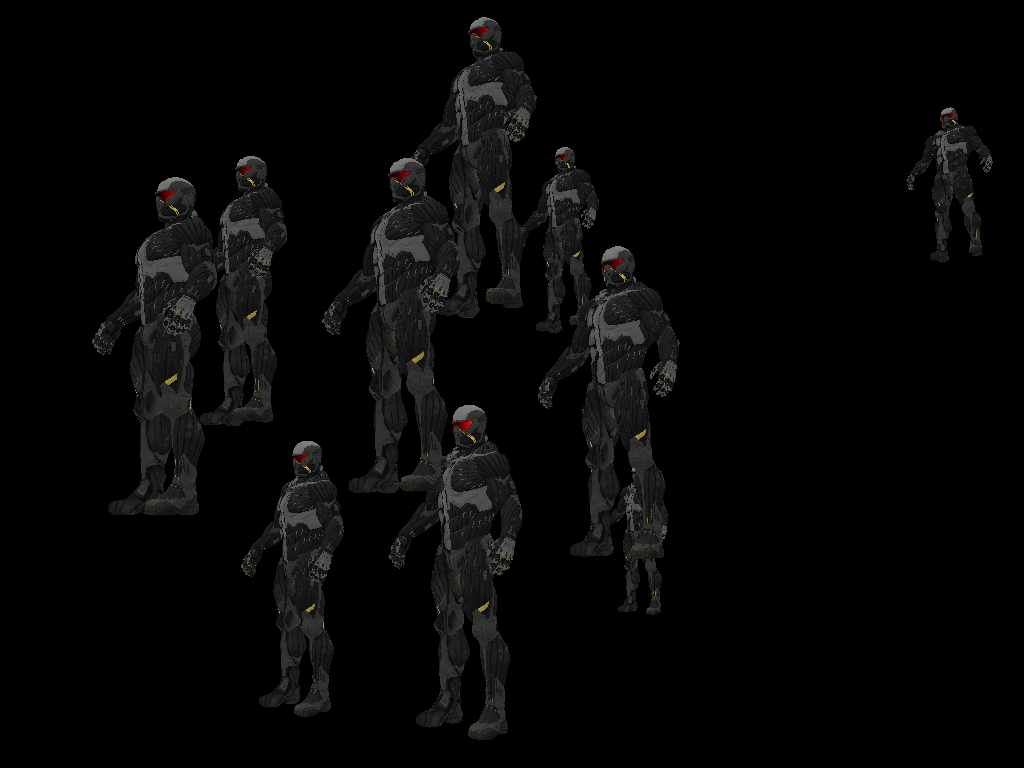
\includegraphics[width=0.32\textwidth]{images/lighting_gBuf_albedoSpec.png}\label{fig:f11}}
  \hfill
  \subfloat[Surface normals]{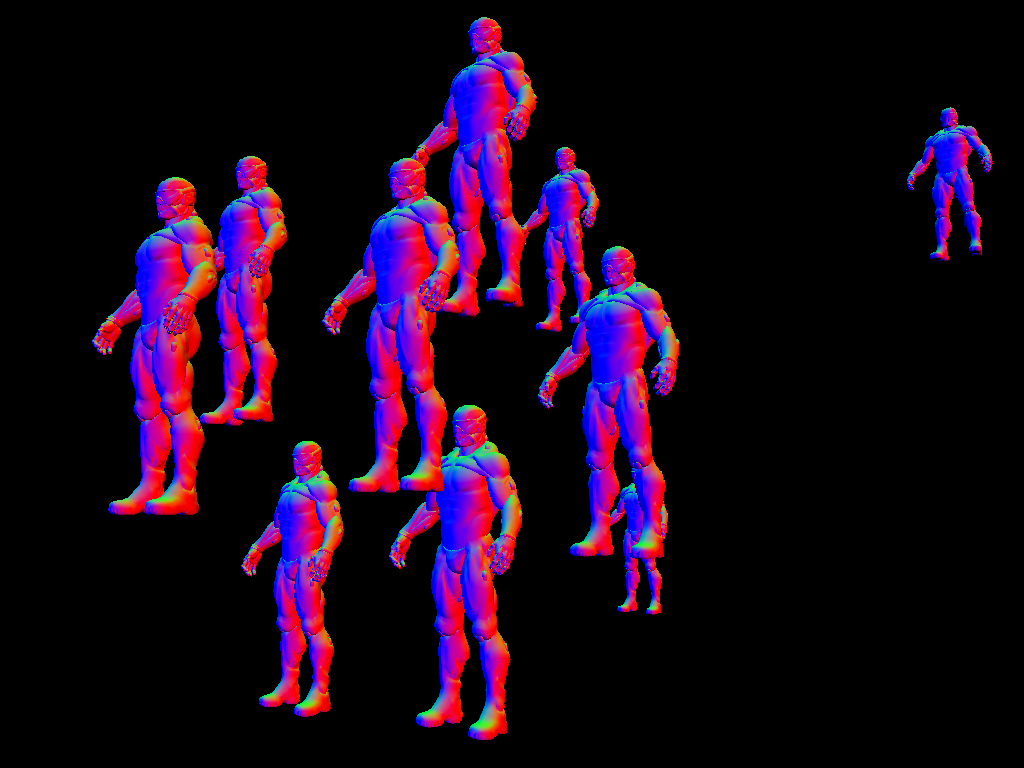
\includegraphics[width=0.32\textwidth]{images/lighting_gBuf_normals.png}\label{fig:f12}}
  \hfill
  \subfloat[Depth]{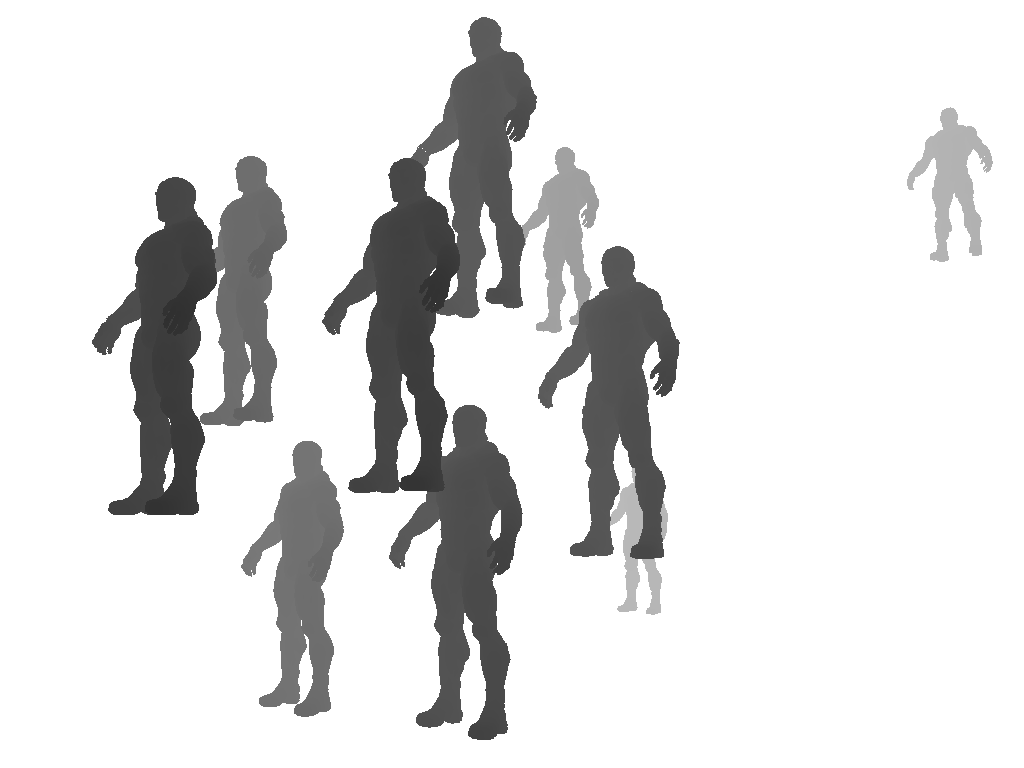
\includegraphics[width=0.32\textwidth]{images/lighting_gBuf_depth.png}\label{fig:f13}}
  \caption{Components of the G buffer in the testbed's deferred shading implementation.}
\end{figure}

Rendering of objects in the scene is performed by a comparatively simple \gls{shader}, which serves to consolidate its inputs, mixing them as appropriate, and writing them to the G buffer. While deferred shading does require a significant amount of additional video memory---particularly since the normal and depth buffers need high precision \glspl{float} to accurately represent their values---it simplifies the lighting processing immensely.

Information about lights, encoded in memory as uniform structures, is sent to a shader, which also takes the G buffer as an input. It performs the necessary calculations for each \gls{texel} and outputs it to the next stage in the rendering pipeline.

\section{Lighting Calculations}
Thanks to the flexibility afforded by performing all lighting calculations at the same time, many different types of lighting can be implemented. In the testbed, four types of lighting are supported: ambient light, directional lights, point lights, and spotlights. Each of these lights has an associated \gls{specular} and \gls{diffuse} colour, among other variables that control its appearance and effect on the scene.

\subsection{Ambient Light}
Ambient light is an average of all non-specific light sources in a scene, with a fixed colour, affecting every \gls{texel} equally. This is typically used to model the way in which thousands of distinct light sources interact to produce the (approximately) same illumination level throughout the scene.

\subsection{Directional Light}
Directional lights are an approximation of light sources that are infinitely far away, modeled as a series of parallel light rays. They have a diffuse and specular colour, and a direction that indicates which way the light rays will be cast. Any \gls{texel} that intersects with a light ray from a directional light will be affected by it.

Directional lights are typically the only lights that will cause shadows to be cast, and as thus, there are very few of them in any given scene.

\subsection{Point Light}
Point lights are similar to directional lights; but rather than a direction, they instead have a specific position. Light rays are cast in all directions from this center point, and like directional lights, any \gls{texel} that intersects such a light ray will be affected by it. Instead of a constant strength, however, the influence of a point light gets weaker the farther the \gls{texel} is from the light source.\footcite{pointlight-attenuate}	

This attenuation is defined by a constant ($K_c$), a linear ($K_l$) and a quadratic ($K_q$) term, as well as the distance from the light ($d$) and unattenuated intensity ($I$): \begin{equation} F_{att} = \frac{I}{K_c + K_l * d + K_q * d^2} \end{equation}

To get the amount of light contributed by a point light towards the final output colour of a \gls{texel}, its specular and diffuse colours are multiplied by $F_{att}$ before mixing.

\subsection{Spotlight}
Spotlights are special cases of point lights, with a direction in addition to a position, as well as a radius. They cast light rays as a cone with a given radius, and illuminate everything that falls within this cone. Toward the edge of the radius, the intensity of the light begins to rapidly decay.

\section{End Result}
When combining all of these types of lighting, a good approximation of a complex environment with many lights can be created.

\begin{figure}[!htbp]
   \centering
   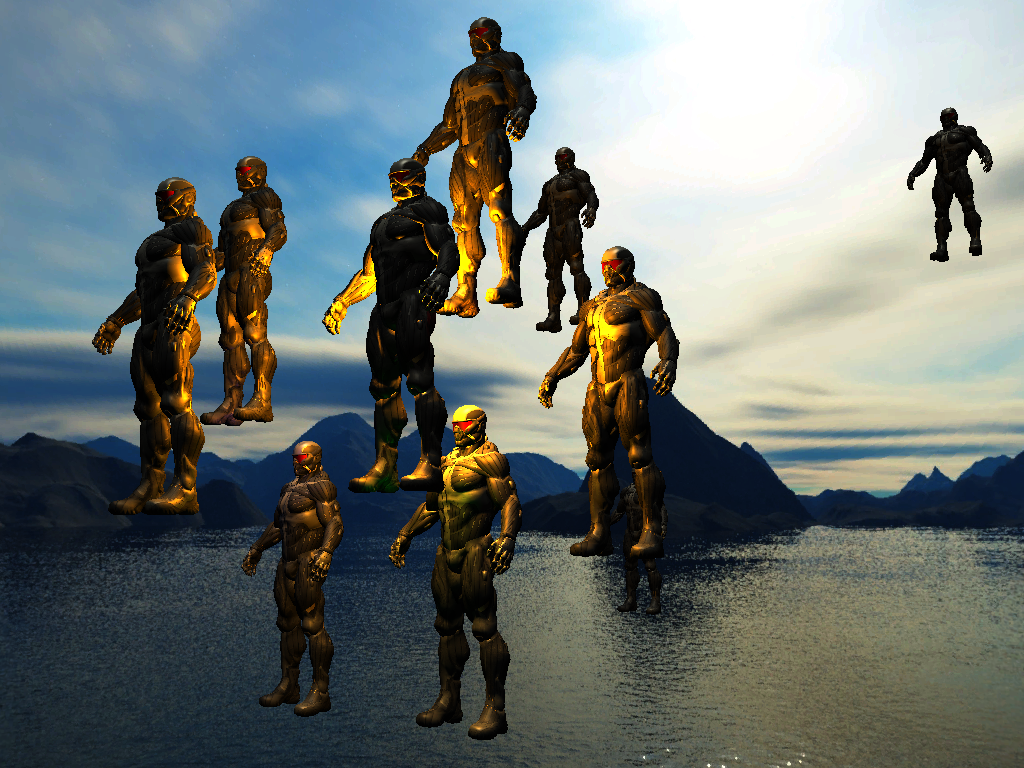
\includegraphics[width=0.74\textwidth]{images/lighting_out.png}
   \caption{Output of the lighting stage, without gamma compensation, with values > \texttt{1.0} clipped. A \gls{skybox} was rendered in areas where lighting calculations produced no output.}
   \label{fig:f14}
\end{figure}

But what about particularly bright lights, or really dark ones? The standard approach to rendering them will cause \glspl{texel} illuminated by them to appear as solid bright or dark areas, losing most detail that may have been present before. \gls{HDR} solves that problem, by having the lighting pass output an intermediate, unbounded representation of light intensity.\footcite{trebilco-deferred}

A downside of deferred shading is that objects that previously affected light in unique ways are more difficult to implement, since all lighting calculations are in the same shader. For example, it becomes very difficult to simulate the way in which a glass vase might distort objects behind it.

Additionally, a significant amount of memory is consumed by the \gls{G Buffer} as compared with regular \gls{forward shading}, so it is not uncommon to reuse components of the \gls{G Buffer} for other purposes.

\subsection{Performance Impact}
By far, deferred shading consumes a significant piece of the frame's processing time. Approximately 9.6\% of the frame processing time goes towards deferred shading. However, compared to the tremendous savings over per-pixel shading, this is still a massive reduction in processing time.

\begin{table}[!htbp]	
	\centering
	\footnotesize
	
	\definecolor{HeaderGray}{gray}{0.74}
		
	\begin{tabularx}{0.88\textwidth}{| r | c | c | >{\tt}X |}	
		\hline
		\rowcolor{HeaderGray}
		\multicolumn{2}{|c|}{Running Time} & Self (ms) & \multicolumn{1}{ c |}{Symbol Name} \\
		\hline
		574.0ms & 9.6\% & 3.0 & {gfx::SceneLighting::render()} \\
		\hline

		356.0ms & 5.9\% & 2.0 & {gfx::SceneLighting::sendLightsToShader()} \\
		89.0ms & 1.4\% & 1.0 & {gl::glDrawArrays(gl::GLenum, int, int)} \\ 
		60.0ms & 1.0\% & 0.0 & {gfx::SceneLighting::renderSkybox()} \\
		20.0ms & 0.3\% & 2.0 & {glm::tmat4x4<float>::inverse} \\[1ex]
		
		13.0ms & 0.2\% & 0.0 & {gfx::ShaderProgram::setUniform1f(std::string, float)} \\
		12.0ms & 0.2\% & 1.0 & {gfx::ShaderProgram::bind()} \\
		5.0ms & 0.0\% & 1.0 & {gfx::Texture2D::bind()} \\
		4.0ms & 0.0\% & 0.0 & {gfx::Texture2D::unbind()} \\[1ex]
		
		3.0ms & 0.0\% & 0.0 & {gfx::ShaderProgram::setUniformVec(std::string, glm::tvec3<float>)} \\
		2.0ms & 0.0\% & 0.0 & <Unknown Address> \\
		2.0ms & 0.0\% & 0.0 & {gfx::ShaderProgram::setUniformMatrix(std::string, glm::tmat4x4<float>)} \\
		1.0ms & 0.0\% & 0.0 & {gfx::VertexArray::unbind()} \\
		\hline
	\end{tabularx}
	
	\caption{Stack trace showing computational impact of deferred shading.}
	\label{tab:booktabs}
\end{table}

Before deferred shading, lighting was calculated for each \gls{texel}. Average frame rendering times sat at approximately 6.3mS, with rendering and lighting consuming a whopping 93.7\% of that time---the majority of which was spent performing complex lighting calculations over texels that would not even be rendered. Implementing deferred shading single-handedly brought the per-frame rendering time down to approximately 2.9mS.

Of the processing overhead incurred by deferred shading, approximately two thirds go towards sending lighting information (such as position, coefficients, colours, etc.) to the lighting shader. Another 10\% go towards rendering a skybox.

As far as memory use goes, deferred shading is relatively resource hungry. Because of the amount of data that is needed for lighting, the \gls{G Buffer} becomes quite large. Three buffers need to be allocated, at full screen resolution---the albedo and specular buffer, a 32 \gls{bpp} integer buffer; the surface normals, a 64 \gls{bpp} floating point buffer; and the depth buffer, a combined depth and stencil floating point format, requiring 32 \gls{bpp}.

An additional 14MB of memory are required for the \gls{G Buffer}. However, all components of the buffer can be reused after the lighting pass for other steps of the rendering pipeline to reduce the overall memory footprint.

\chapter{High Dynamic Range (HDR) and Bloom}
One of the biggest problems of computer graphics has traditionally been to approach the dynamic range of the human eye, even though display devices have a limited colour palette they can reliably and accurately display. Particularly, the human eye is much better at recovering detail from very bright and very dark areas than a computer display can show, so a large range of brightness values must somehow be mapped onto the handful of nonlinear brightness values displayed by computer monitors: this is exactly what \gls{HDR} does, via a process called \gls{tone mapping}.

Additionally, due to optical imperfections in lenses (the eye is really one big lens) there often appears bleeding of light from very bright to darker areas. By applying \gls{bloom}, the brightness of a light source can be exaggerated and shown more clearly.

\section{Producing HDR Output}
The deferred shading pass outputs colour values into a \gls{floating point} buffer, allowing for a nearly infinite amount of brightness values to be expressed. The conversion between HDR values and \gls{RGB} values is relatively straightforward, and is defined by a function in a \gls{shader}; also known as \gls{tone mapping}. These values are also adjusted to match a certain \gls{white point}\footcite{hdr}.

\begin{figure}[!htbp]
  \centering
  \subfloat[Before]{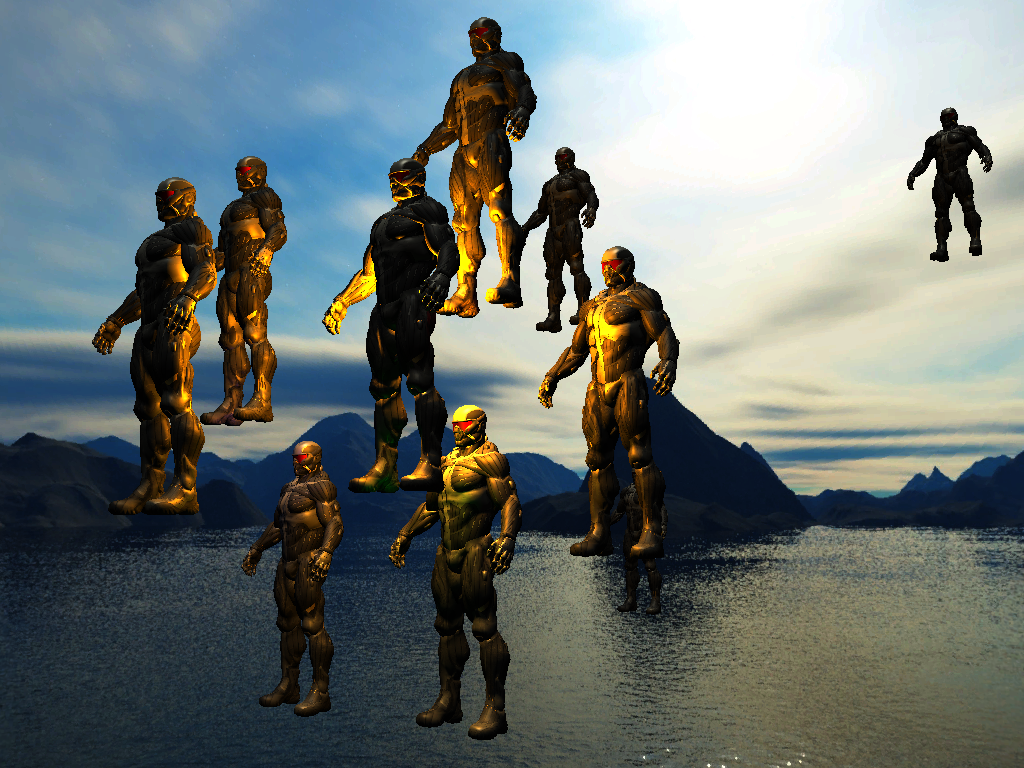
\includegraphics[width=0.49\textwidth]{images/lighting_out.png}\label{fig:f21}}
  \hfill
  \subfloat[After]{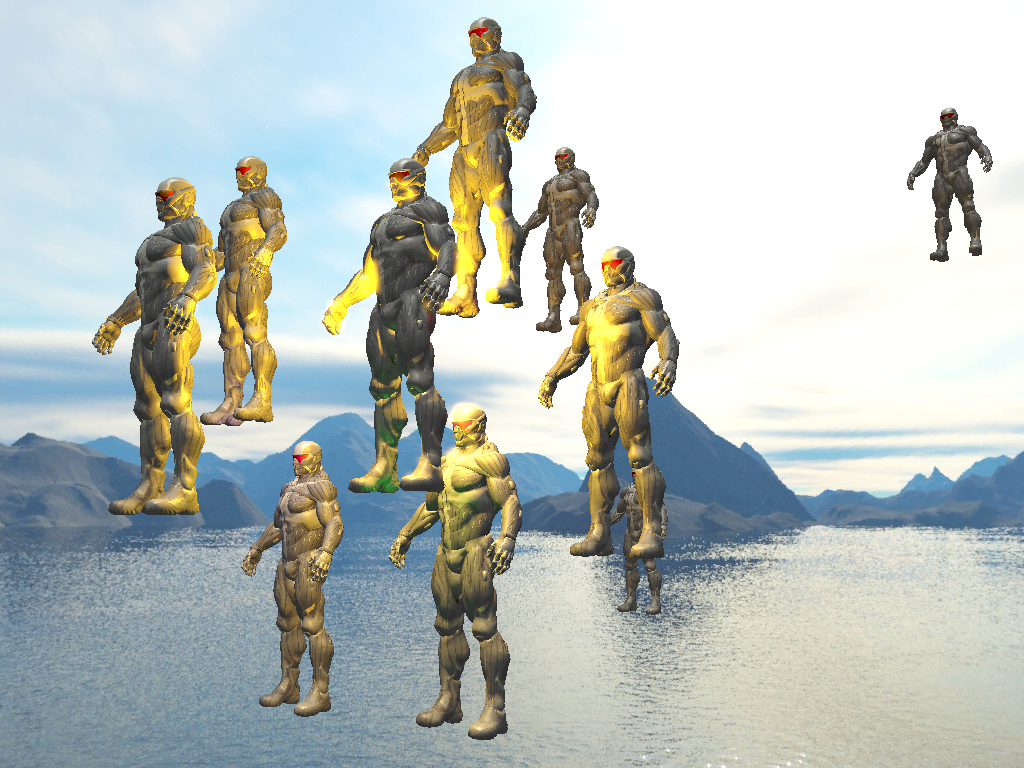
\includegraphics[width=0.49\textwidth]{images/bloom_hdr_out.png}\label{fig:f22}}
  \caption{Before and after \gls{tone mapping}, gamma and white point adjustments.}
\end{figure}

In addition to a particular \gls{tone mapping} algorithm, the sensitivity of \gls{HDR} can easily be adjusted via an exposure parameter. This parameter serves as a constant multiplier for the \gls{HDR} input colours before \gls{tone mapping}, and affects the overall brightness of the image: similarly to how changing the exposure settings on a photographic camera will affect the brightness of the resultant image.

\begin{figure}[!htbp]
  \centering
  \subfloat[-3]{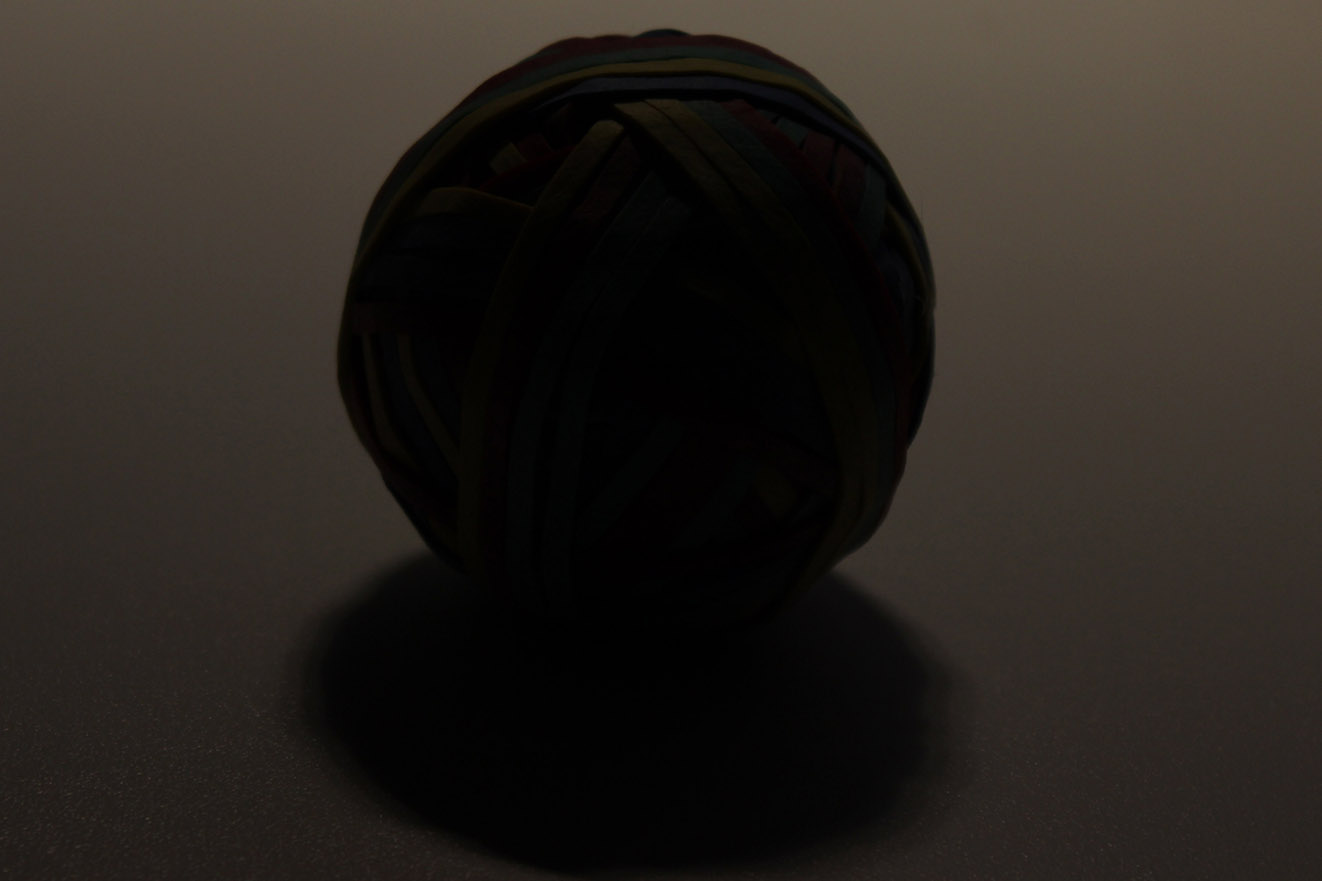
\includegraphics[width=0.19\textwidth]{images/exposure/EV_-3.jpg}\label{fig:f23}}
  \hfill
  \subfloat[-1.5]{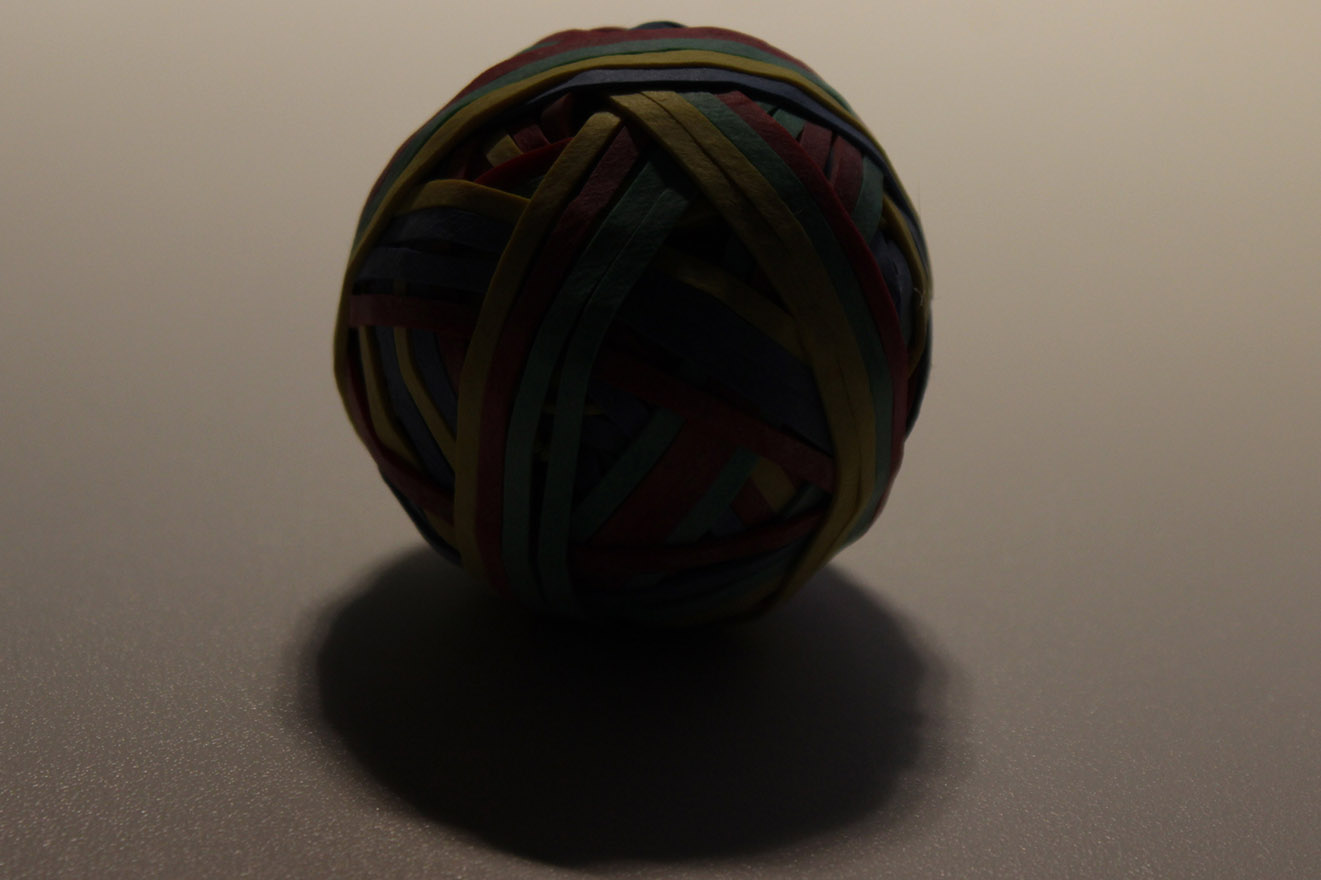
\includegraphics[width=0.19\textwidth]{images/exposure/EV_-1_5.jpg}\label{fig:f24}}
  \hfill
  \subfloat[0]{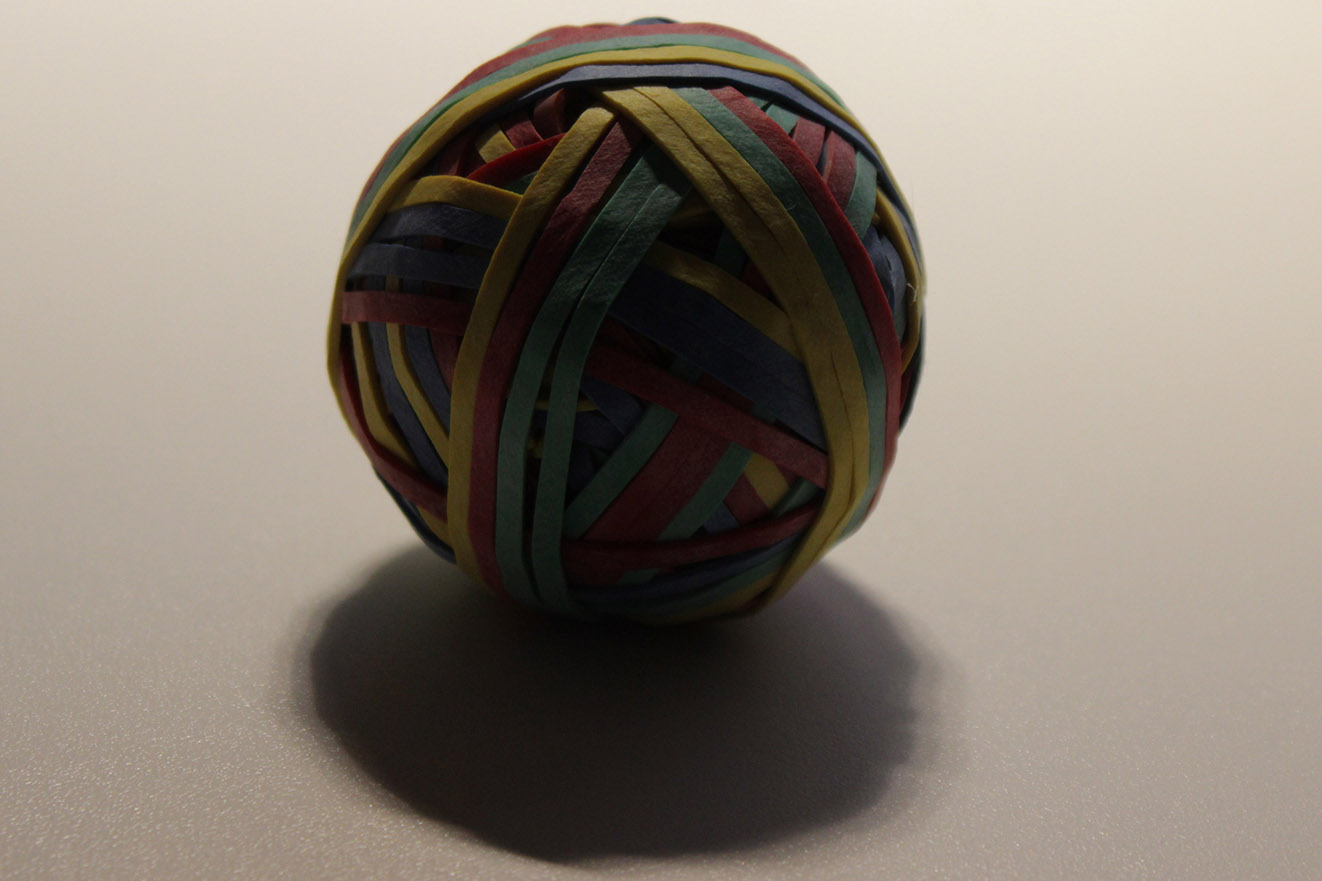
\includegraphics[width=0.19\textwidth]{images/exposure/EV_0.jpg}\label{fig:f25}}
  \hfill
  \subfloat[1.5]{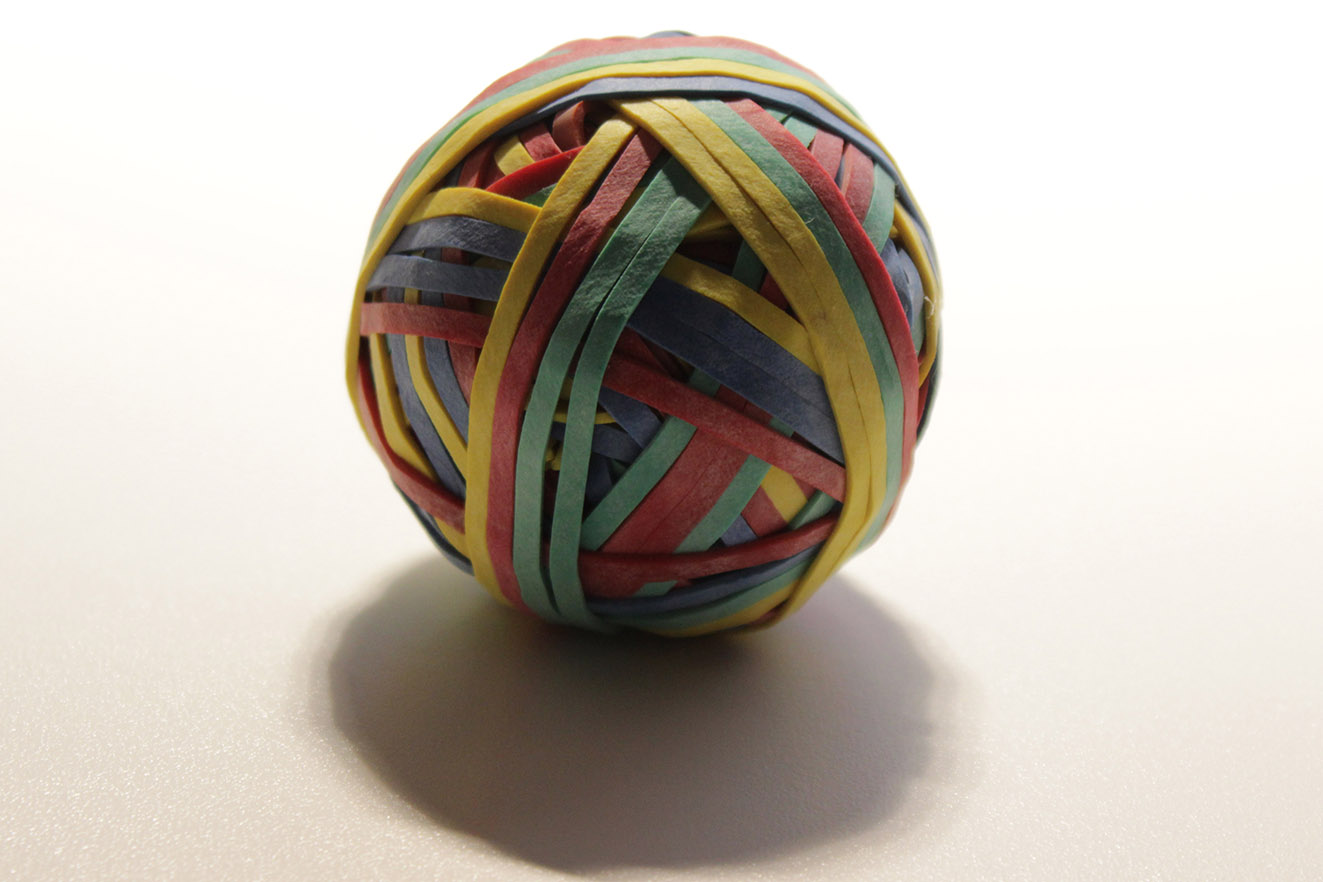
\includegraphics[width=0.19\textwidth]{images/exposure/EV_1_5.jpg}\label{fig:f26}}
  \hfill
  \subfloat[3]{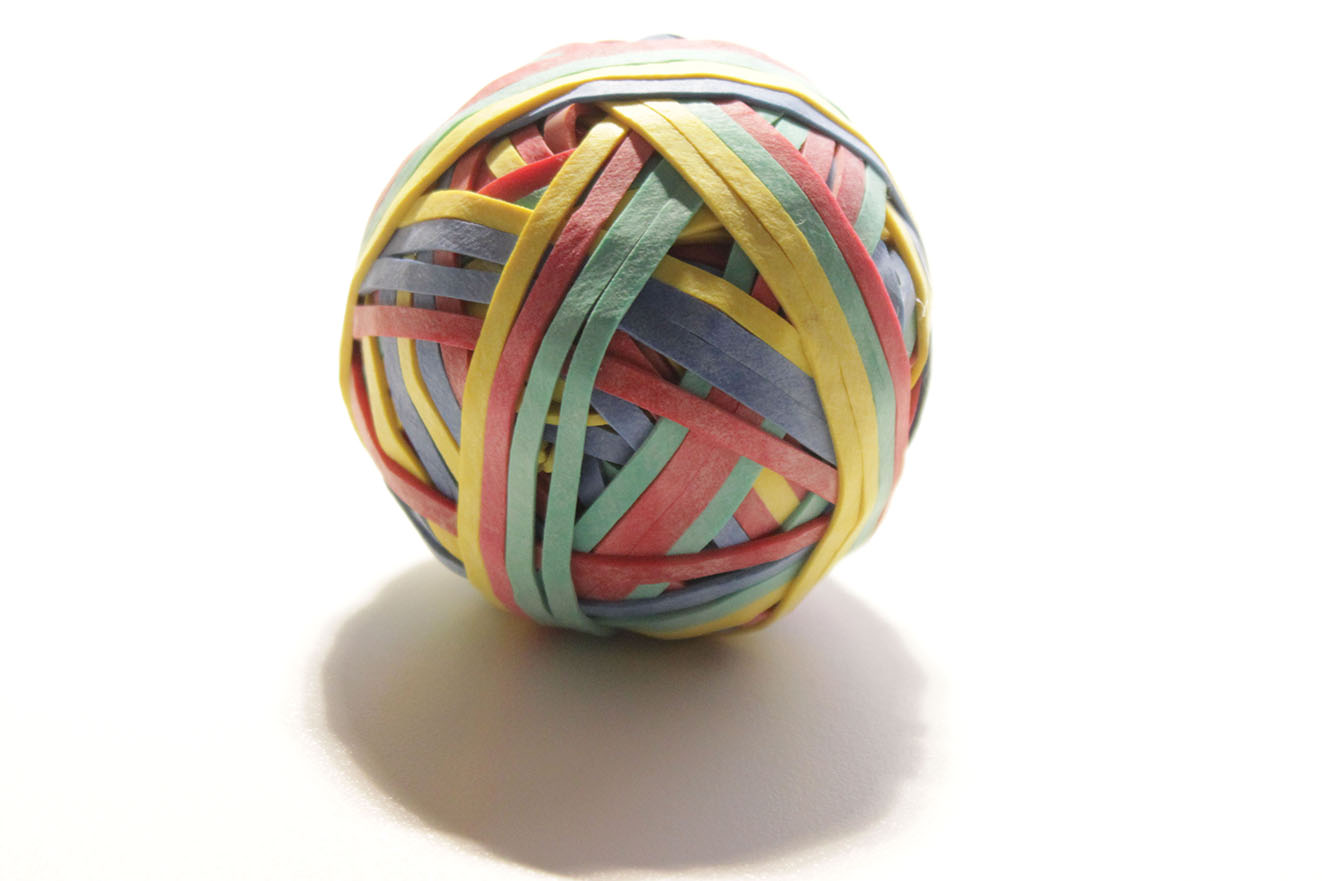
\includegraphics[width=0.19\textwidth]{images/exposure/EV_3.jpg}\label{fig:f27}}
  \caption{Effects of varying exposure values (EV) on a photograph.}
\end{figure}

Overall, HDR can produce a great improvement in visual quality with little additional work. An extra stage of shader processing before output adds minimal overhead, and no additional memory is needed, if a buffer from a previous stage in the rendering pipeline can be reused.

Various additional effects can be achieved simply by varying the exposure value: for example, a higher exposure value could be used for night-time scenes, and a lower one for day-time scenes. Perhaps even automatic exposure adjustment, where the overall brightness is analyzed, and exposure is slowly changed to maintain a baseline level of brightness, similar to how the human eye functions---temporary blindness when going from a dark scene to a bright scene, or vice-versa, while the eye slowly adjusts to the difference in average brightness.

\section{Bloom}
Blooming simulates the glow that occurs around extremely bright light sources. In conjunction with \gls{HDR}, it is incredibly easy to implement, incuring little additional overhead---but significantly increases the photorealism if implemented properly.

\begin{figure}[!htbp]
  \centering
  \subfloat[Before]{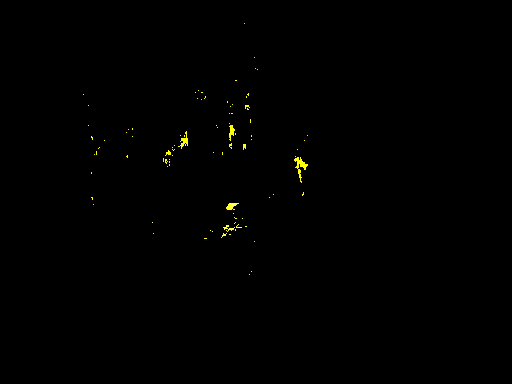
\includegraphics[width=0.49\textwidth]{images/bloom_bright_in.png}\label{fig:f28}}
  \hfill
  \subfloat[After]{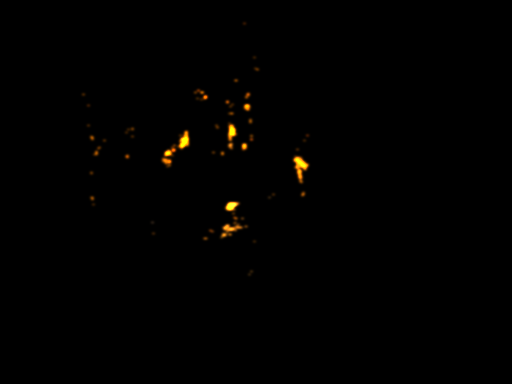
\includegraphics[width=0.49\textwidth]{images/bloom_pass4.png}\label{fig:f29}}
  \caption{Bright input fragments, before and after application of the Gaussian blur.}
\end{figure}

All fragments that are considered bright---a combined brightness of \texttt{1.0} or above---are copied into an additional buffer. This buffer is half the size as the output screen, thus saving memory and processing time. A second buffer of identical size is allocated. This buffer is then blurred through several iterations of a Gaussian blur, until an adequate blur has been achieved.\footcite{gpupro-hdr}

The Gaussian blur itself consists of a $13 \times 13$ blur kernel, which is approximated by sampling the texture seven times for each \gls{texel}, using bilinear interpolation to simulate the effect of sampling many more times. The blur itself has been decomposed into separate horizontal and vertical components for performance reasons---a performance impact of $O(n)$ rather than $O(n^2)$---and is run over a set of two buffers: the original 'bright fragment' input buffer, and the eventual 'output' buffer a predetermined number of times. Once blurring has been completed, the output buffer is sampled in the \gls{HDR} output shader, multiplied by a coefficient (this determines the strength and effect of the blur on the rest of the scene,) then added to the calculated \gls{HDR} colour.

\section{End Result}
By combining both \gls{HDR} and blooming, the lighting in a scene already appears much more realistic, solving the issue of washed out highlights and details that disappear into the shadows. These two render passes require little in the way of additional memory, and their \gls{shader} programs are relatively simple, compared to various other techniques. 

Additionally, the \gls{HDR} pass serves as a place for gamma correction to take place. Textures are stored as sRGB, and \gls{OpenGL}'s built-in conversion is disabled. This way, the user can configure the gamma of the application to match their monitor most closely, instead of relying on a hard-coded value in a graphics driver, or relying on the operating system to get it right.

\subsection{Performance Impact}
\begin{table}[!htbp]	
	\centering
	\footnotesize
	
	\definecolor{HeaderGray}{gray}{0.74}
	\definecolor{Header2Gray}{gray}{0.95}
		
	\begin{tabularx}{0.88\textwidth}{| r | c | c | >{\tt}X |}	
		\hline
		\rowcolor{HeaderGray}
		\multicolumn{2}{|c|}{Running Time} & Self (ms) & \multicolumn{1}{ c |}{Symbol Name} \\
		
		\hline
		\rowcolor{Header2Gray}
		\multicolumn{4}{|c|}{\textbf{HDR}} \\
		\hline
		103.0ms & 1.7\% & 0.0 & {gfx::HDRRenderer::render()} \\
		\hline
		
		92.0ms & 1.5\% & 0.0 & {gl::glDrawArrays(gl::GLenum, int, int)} \\
		5.0ms & 0.0\% & 0.0 & {gfx::ShaderProgram::bind()} \\
		3.0ms & 0.0\% & 0.0 & {gfx::VertexArray::bind()} \\
		2.0ms & 0.0\% & 0.0 & {gfx::Texture2D::bind()} \\
		
		\hline
		\rowcolor{Header2Gray}
		\multicolumn{4}{|c|}{\textbf{Bloom}} \\
		\hline
		127.0ms & 2.1\% & 0.0 & {gfx::BloomRenderer::render()} \\
		\hline
		
		103.0ms & 1.7\% & 0.0 & {gl::glDrawArrays(gl::GLenum, int, int)} \\
		10.0ms & 0.1\% & 1.0 & {gfx::ShaderProgram::bind()} \\
		10.0ms & 0.1\% & 0.0 & {gfx::ShaderProgram::setUniform1i(std::string, int)} \\
		2.0ms & 0.0\% & 0.0 & {gfx::ShaderProgram::setUniform1f(std::string, float)} \\[1ex]
		
		2.0ms & 0.0\% & 0.0 & {gfx::ShaderProgram::setUniformVec(std::string, glm::tvec3<float>)} \\


		\hline
	\end{tabularx}
	
	\caption{Stack trace showing computational impact of HDR and blooming.}
	\label{tab:booktabs}
\end{table}

When analyzing the testbed's performance with \gls{HDR} and blooming enabled, the relatively insignificant additional overhead incurred by the technique immediately becomes clear.

After optimizing the \gls{HDR} code to reduce \glspl{pipeline stall}, on average, 1.7\% of a frame's processing time was taken up by the blurring of highlights (for blooming) and the combination and \gls{tone mapping} of the final output.

In addition, 6.2MB of video memory were needed for buffers. The two quarter resolution buffers for blooming are 48 \gls{bpp} floating point buffers without alpha components, while the input buffer to the HDR process is a 64 \gls{bpp} floating point buffer.

Considering the improvement in visual quality that a properly implemented \gls{HDR} approach can give, the additional performance overhead is almost negligible. However, the difficulty lies in determining and implementing a good \gls{tone mapping} algorithm, that gives an output that looks realistic---not too saturated, but not too bland, either.

Furthermore, a topic of much discussion in the CGI community is blooming. It is extremely difficult to come up with a bloom threshold that is appropriate for every environment where photorealistic rendering is desired, so it is often times determined experimentally, and varies from scene to scene.

\chapter{Fast Approximate Antialiasing (FXAA)}
Due to the limited resolution of textures and other data, as well as the multitude of transformations applied to geometric primitives, it is extremely common for an unprocessed render output to exhibit heavy \gls{aliasing}. Often, \gls{aliasing} takes the form of jagged edges, but it can also manifest itself as strange and unnatural transitions between colours, contributing extremely negatively toward the quality of the rendered image.

In the past, aliasing was combatted by rendering the entire scene at a much higher resolution---often 2x or 4x larger than the physical display resolution---then simply downscaling it, creating a primitive form of \gls{supersampling}. Later on, similar techniques were applied to \glspl{shader}, causing \gls{multisampling} to take place when they sampled textures, not when they produced their output, improving performance somewhat; also known as MSAA. Supersampling works in a similar manner.

What all of these antialiasing algorithms have in common is that they are very computationally expensive. They can double or quadruple the rendering time, while yielding a minimal benefit.

\section{Implementation}
Processing the output with \gls{FXAA} is straightforward. A buffer is created, into which the output of all previous stages of the rendering pipeline is stored, instead of directly going to the window framebuffer. This buffer is then set as an input to the \gls{FXAA} \gls{shader} program, which samples it, detects edges, smoothes them, and outputs a final antialiased output to the window framebuffer\footcite{nvidia-fxaa}.

\begin{figure}[!htbp]
  \centering
  \subfloat[With FXAA]{
\includegraphics[width=0.49\textwidth]{images/fxaa_out@8x.png}\label{fig:f31}}
  \hfill
  \subfloat[Without FXAA]{
\includegraphics[width=0.49\textwidth]{images/bloom_hdr_out@8x.png}\label{fig:f32}}
  \caption{A crop from the final output, with and without FXAA. Note the rough edges on on (b).}
\end{figure}

Because \gls{FXAA} is implemented in a shader\footnote{Example implementation from NVIDIA, Version 3.11 by Timothy Lottes}, rather than in hardware, its behavior (such as edge detection sensitivity, smoothing algorithm and sharpness, etc.) can be adjusted on-the-fly by the user to produce the quality of output they desire.

\section{End Result}
By utilizing a new algorithm to approximate antialiasing instead of wasting precious computational resources and \gls{memory bandwidth} on traditional algorithms, immense performance gains can be had. In most cases, the quality of \gls{FXAA} is comparable to that of more traditional antialiasing algorithms: and most of the time, the precise nature of the antialiasing algorithm makes little difference to the user of the program, so long as \gls{aliasing} artifacts are minimized.

\subsection{Performance Impact}
Implementing \gls{FXAA} improves the quality of the output significantly, by removing \gls{aliasing} artifacts, with little impact on the performance of the rendering pipeline.

\begin{table}[!htbp]	
	\centering
	\footnotesize
	
	\definecolor{HeaderGray}{gray}{0.74}
		
	\begin{tabularx}{0.88\textwidth}{| r | c | c | >{\tt}X |}	
		\hline
		\rowcolor{HeaderGray}
		\multicolumn{2}{|c|}{Running Time} & Self (ms) & \multicolumn{1}{ c |}{Symbol Name} \\
		\hline
		127.0ms & 2.1\% & 0.0 & {gfx::FXAARenderer::render()} \\
		\hline
		
		101.0ms & 1.6\% & 0.0 & {gl::glDrawArrays(gl::GLenum, int, int)} \\
		10.0ms & 0.1\% & 2.0 & {gfx::ShaderProgram::setUniform1f(std::string, float)} \\
		10.0ms & 0.1\% & 0.0 & {gfx::ShaderProgram::setUniform1i(std::string, int)} \\
		5.0ms & 0.0\% & 0.0 & {gfx::ShaderProgram::bind()} \\[1ex]
		
		1.0ms & 0.0\% & 0.0 & {gfx::Texture2D::bind()} \\
		\hline
	\end{tabularx}
	
	\caption{Stack trace showing computational impact of deferred shading.}
	\label{tab:booktabs}
\end{table}

On average, running the \gls{FXAA} pass, using the highest 'low dither' preset specified by the shader, 2.1\% of  processing time is required to execute the \gls{FXAA} algorithm each frame. The majority of this time is spent in the \gls{OpenGL} library, waiting for the GPU to be ready to accept a command, so there is room for further optimization.

In addition, another colour buffer is needed, increasing memory overhead by approximately 4MB. (A simple 24 \gls{bpp} buffer without alpha will suffice for this application, since all \gls{HDR} processing will have already been done on the more complex buffers.)

For the improvement in visual quality---in particular, when using large output displays, and the low impact on performance---the impact of implementing \gls{FXAA} is basically nil.

However, it is important to consider the impact that \gls{FXAA} might have on various graphical overlays, such as HUDs, or various user interface elements. Often times, unexpected artifacts are created when \gls{FXAA} works on such overlays, so they would be rendered in another buffer, and then overlaid on the output of the \gls{FXAA} shader.

\chapter{Overall Performance}
To determine the overall effect on performance of the aforementioned rendering techniques, Apple's Instruments software was used to capture stack traces, and combining those with timing information within the testbed itself.

\begin{table}[!htbp]
	\centering
	\footnotesize
	
	\definecolor{HeaderGray}{gray}{0.74}
		
	\begin{tabularx}{0.88\textwidth}{| r | c | c | >{\tt}X |}	
		\hline
		\rowcolor{HeaderGray}
		\multicolumn{2}{|c|}{Running Time} & Self (ms) & \multicolumn{1}{ c |}{Symbol Name} \\
		\hline
		5956.0ms & 100.0\% & 3.0 & {gfx::StandardRenderer::render()} \\
		4021.0ms & 67.5\% & 5.0 & {gfx::SceneRenderer::render()} \\
		574.0ms & 9.6\% & 3.0 & {gfx::SceneLighting::render()} \\
		531.0ms & 8.9\% & 0.0 & {gfx::BloomRenderer::beforeRender()} \\[1ex]
		205.0ms & 3.4\% & 0.0 & {gfx::SceneRenderer::beforeRender()} \\
		127.0ms & 2.1\% & 0.0 & {gfx::BloomRenderer::render()} \\
		127.0ms & 2.1\% & 0.0 & {gfx::FXAARenderer::render()} \\
		103.0ms & 1.7\% & 0.0 & {gfx::HDRRenderer::render()} \\[1ex]
		96.0ms & 1.6\% & 0.0 & {gfx::SceneLighting::beforeRender()} \\
		57.0ms & 0.9\% & 0.0 & {gfx::SceneRenderer::renderNormally()} \\
		43.0ms & 0.7\% & 1.0 & {gfx::SceneLighting::bindGBuffer()} \\
		19.0ms & 0.3\% & 0.0 & {gfx::LevelCamera::updateViewMatrix()} \\[1ex]
		18.0ms & 0.3\% & 0.0 & <Unknown Address> \\
		8.0ms & 0.1\% & 0.0 & {gfx::HDRRenderer::bindHDRBuffer()} \\
		3.0ms & 0.0\% & 0.0 & {gfx::BloomRenderer::bindBloomBuffer()} \\
		3.0ms & 0.0\% & 1.0 & {gfx::FXAARenderer::beforeRender()} \\[1ex]
		2.0ms & 0.0\% & 0.0 & {gfx::FrameBuffer::unbindRW()} \\
		2.0ms & 0.0\% & 0.0 & {gfx::HDRRenderer::beforeRender()} \\
		2.0ms & 0.0\% & 0.0 & {gfx::LevelCamera::getViewMatrix()} \\
		1.0ms & 0.0\% & 1.0 & {glm::detail::tmat4x4<float>::tmat4x4()} \\[1ex]
		1.0ms & 0.0\% & 0.0 & {gfx::LevelCamera::getCameraLookAt()} \\
		1.0ms & 0.0\% & 0.0 & {gfx::SceneLighting::setFXAA(gfx::FXAARenderer*)} \\
		1.0ms & 0.0\% & 0.0 & {gfx::LevelCamera::getCameraPosition()} \\
		1.0ms & 0.0\% & 0.0 & {gfx::SceneRenderer::afterRender()} \\[1ex]
		1.0ms & 0.0\% & 0.0 & {gfx::FXAARenderer::bindFXAABuffer()} \\
		1.0ms & 0.0\% & 0.0 & {gfx::SceneLighting::afterRender()} \\
		\hline
	\end{tabularx}
	
	\caption{Stack trace showing each step of the rendering pipeline, after running it for 60 seconds.}
	\label{tab:booktabs}
\end{table}

The implementation of these techniques does indeed affect the quality of the output in a positive way. Deferred shading allows for many more lights, giving a more realistic model of how light interacts with objects in the real world. \gls{HDR} and blooming more accurately model the way in which the human eye perceives light, matching its dynamic range, and emulating some of its imperfections. \gls{FXAA} smoothes the final output, getting rid of unpleasant rendering artifacts without the excessive overhead of previous methods antialiasing or \gls{supersampling}.

However, these gains in appearance are not entirely free. While deferred shading reduces processing time required for each \gls{texel} significantly, it requires a significant amount of memory to store the additional data required to later render the lighting effects.

\gls{HDR} and \gls{FXAA} require additional memory as well, but provide an incredible increase in the quality of the output with little additional processing time required.

While these basic techniques by themselves do not magically create photorealistic outputs, they are significant steps towards allowing for much more complex shaders, and other processing techniques, that allow true photorealism. For example, dynamic reflections and shadows could be used to enhance the appearance of objects. More complex and detailed textures and normal maps could allow rendered objects to have more detail than the mesh used to render them really does.

Overall, these techniques do contribute quite significantly to the appearance and quality of the final output. While they by themselves do not achieve photorealism, they definitely serve as important foundations for achieving photorealism.

An effective base of low-overhead techniques that can be extended at a later time are necessary for more advanced techniques---such as ambient occlusion or 3D shadow mapping---to build on.
	
\begingroup	
	\setlength\bibitemsep{18pt}

	\printbibliography[
		heading=bibintoc,
		title={Bibliography}
	]
\endgroup

\printglossaries

\begin{landscape}

\end{landscape}

\end{document}